\subsection{Diagramma della fase}
Per presentare il diagramma della fase si riporta la funzione di trasferimento
nella forma di Bode
$$
W(s) = \frac{K_B}{(s)^g}\cdot \frac{\prod_i (1+s \tau_{zi})
\prod_i \left(1+\frac{s^2}{\omega_{nz_i}^2} +
\frac{2\zeta_{zi}}{\omega_{nz_i}}s\right) }
{\prod_i (1+s \tau_{pi})
\prod_i \left(1+\frac{s^2}{\omega_{np_i}^2} +
\frac{2\zeta_{pi}}{\omega_{np_i}}s\right) }
$$
Si studia la funzione sull'asse immaginario ossia quando $s=j\omega$
$$
W({j\omega}) = \frac{K_B}{({j\omega})^g}\cdot \frac{\prod_i (1+{j\omega}
\tau_{zi})
\prod_i \left(1-\frac{\omega^2}{\omega_{nz_i}^2} +
\frac{2\zeta_{zi}}{\omega_{nz_i}}\omega j\right) }
{\prod_i (1+{j\omega} \tau_{pi})
\prod_i \left(1-\frac{\omega^2}{\omega_{np_i}^2} +
\frac{2\zeta_{pi}}{\omega_{np_i}}\omega j\right) }$$

Si ricordano le proprietà della fase: la fase del prodotto è la somma delle
fasi, la fase del rapporto è la differenza delle fasi.

$$\begin{aligned}
\phase{W(j\omega)} &= \phase{K_B} - g\phase{j\omega} +
\sum_i\phase{1+j\omega\tau_{z_i}} +
\sum_i\phase{1-\frac{\omega^2}{\omega_{nz_i}^2}+\frac{2\zeta_{zi}}{\omega_{nz_i}
}\omega j} - \\
&-\sum_i\phase{1+j\omega\tau_{p_i}} -
\sum_i\phase{1-\frac{\omega^2}{\omega_{np_i}^2} +
\frac{2\zeta_{pi}}{\omega_{np_i}}\omega j}
\end{aligned}$$
Anche per la fase si può fare prima un diagramma asintotico e poi applicare le
correzioni.
$$
W_a(j\omega) = K_B,\ W_b(j\omega) = \frac{1}{j\omega},\
W_c(j\omega)=\frac{1}{1+j\omega_\tau},\ W_d(j\omega) =
\frac{1}{1-\frac{\omega^2}{\omega_n^2}+j\frac{2\zeta}{\omega_n}\omega}
$$

\textbf{Fase del guadagno} \`E un numero reale dunque la sua fase può essere 0
o -180\textdegree
$$
\phase{W_a(j\omega)} = \phase{K_B} \left\langle
\begin{aligned}
& 0 & & K_b > 0 \\
& \SI{-180}{\degree} & & K_B <0
\end{aligned}\right.
$$
\begin{figure}[h]
\centering
\begin{tikzpicture}[
gnuplot def/.append style={prefix={tikz/}}]
\begin{scope}[xscale=7/3,yscale=3/180]
\tikzset{
semilog lines/.style={black},
}
\OrdBode{30}
\UniteDegre
\semilog{-1}{2}{-180}{0}
\BodeGraph[samples=2]{-1:2}{-180}
\BodeGraph[samples=2]{-1:2}{0}
\end{scope}
\end{tikzpicture}
%\caption{$\textcolor{red}{\zeta=\zOne},\quad \textcolor{blue}{\zeta=\zTwo} $}
\end{figure}

\newpage
\textbf{Fattore monomiale} Un polo nell'origine ha un comportamento costante
pari a -$g$90\textdegree\ in base al tipo di sistema si ha un ritardo di fase
$$
\phase{W_b(j\omega)} = \phase{\frac{1}{(j\omega)^g}} = -g\SI{90}{\degree}
$$
Uno zero nell'origine introdurrà invece un anticipo di fase

\textbf{Termine binomio}
$$
\phase{W_c(j\omega)} = \phase{\frac{1}{1+j\omega \tau}} =
-\phase{1+j\omega\tau} = -\arctan(\omega\tau)
$$
L'analisi asintotica
$$
\phase{W_c(j\omega)} \simeq \left\{
\begin{aligned}
&-\phase{1}= 0 & & & \omega \ll \frac{1}{|\tau|} \\
&-\phase{j\omega\tau} = \left\{
\begin{aligned}
&\SI{-90}{\degree} & &\tau> 0 \\
&\SI{90}{\degree} & & \tau<0
\end{aligned}\right. & & & \omega \gg \frac{1}{|\tau|}
\end{aligned}\right.
$$

\begin{figure}[h]
\centering
\begin{tikzpicture}[
gnuplot def/.append style={prefix={tikz/}}]
\begin{scope}[xscale=7/3,yscale=3/180]
\tikzset{
semilog lines/.style={black},
}
\OrdBode{15}
\UniteDegre
\semilog{-1}{2}{-90}{90}
\BodeGraph[asymp lines,samples=2000]{-1:2}{\POArgAsymp{1}{0.5}}
\BodeGraph[samples=100]{-1:2}{\POArg{1}{0.5}}
\BodeGraph[asymp lines,samples=2000,color=red]{-1:2}{-\POArgAsymp{1}{0.333}}
\BodeGraph[samples=100,color=red]{-1:2}{\POArg{1}{-0.333}}
\end{scope}
\end{tikzpicture}
\caption{$\textcolor{red}{\tau=<0},\quad
\textcolor{blue}{\tau=>0} $}
\end{figure}
Nel punto di rottura si introduce l'inversione del livello della fase.
Un punto di correzione certo è il passaggio a $\frac{1}{\tau}$ pari a $\pm
\SI{45}{\degree}$. Se ci si riferisce ad uno zero anziché un polo si ribalta il
grafico.
Anche in questo caso il fattore esponenziale $g$ moltiplica la funzione
scalando il valore degli asintoti a 180 per $g=2$ e così via.

\newpage
\textbf{Fattore trinomio}
$$
\phase{W_d(j\omega)}  = -
\phase{1-\frac{\omega^2}{\omega_n^2}+j\frac{2\zeta}{\omega_n}\omega}
$$
Si ricorda che $-1<\zeta<1$, si studia il caso limite $\zeta=0$ ossia due poli
puramente immaginari
$$
W_d(j\omega) = \frac{1}{1-\frac{\omega^2}{\omega_n^2}} = \left\{
\begin{aligned}
 &> 0 &  & \omega < \omega_n\\
 &< 0 &  & \omega > \omega_n
\end{aligned}
\right.
$$
\begin{figure}[h]
\centering
\begin{tikzpicture}[
gnuplot def/.append style={prefix={tikz/}}]
\begin{scope}[xscale=7/3,yscale=3/180]
\tikzset{
semilog lines/.style={black},
}
\OrdBode{30}
\UniteDegre
\semilog{-1}{2}{-180}{0}
\BodeGraph[samples=2000]{-1:2}{\SOArgAsymp{1}{0}{3}}
\BodeGraph[samples=100,color =red]{-1:2}{\SOArg{1}{1}{3}}

\end{scope}
\end{tikzpicture}
\caption{$\textcolor{blue}{\zeta=0},\quad
\textcolor{red}{\zeta=1} $}
\end{figure}

Se invece $\zeta=1$ si ricade nel caso di due fattori binomiali coincidenti,
si ottiene una curva passante per $\SI{-90}{\degree}$.
Se $\zeta$ fosse negativo si invertirebbe ancora una volta il grafico, con
asintoto a \SI{+180}{\degree} e punto intermedio a \SI{+90}{\degree}.
Con gli zeri si inverte il grafico.

Si espongono le regole di tracciamento per il diagramma di fase. La prima parte
coincide con quella vista nel diagramma dei moduli
\begin{enumerate}
 \item Per pulsazioni molto piccole, minori del primo punto di rottura, gli
unici contributi sono dati dal guadagno (se negativo) e da eventuali poli
centrati nell'origine, l'ordinata iniziale sarà a quota pari a $\phase{K_B}
-g\cdot\SI{90}{\degree}$
 \item In corrispondenza di punti di rottura di poli o zeri reali, l'ordinata
aumenta $(\tau_p<0,\tau_z>0)$ o diminuisce $(\tau_p>0,\tau_z<0)$ di
$\SI{90}{\degree}\cdot m_a$
\item In corrispondenza di punti di rottura di poli o zeri complessi,
l'ordinata aumenta $(\zeta_p<0,\zeta_z>0)$ o diminuisce $(\zeta_p>0,\zeta_z<0)$
di $\SI{180}{\degree}\cdot m_a$
\end{enumerate}

\newpage
Si riporta il diagramma in frequenza della funzione studiata a pag.
\pageref{sec:Esercizio_bode}
\begin{figure}[h]
\centering
\begin{tikzpicture}[xscale=7/3,
gnuplot def/.append style={prefix={tikz/}}]
\begin{scope}[yscale=3/60]
\tikzset{
semilog lines/.style={black},
}
\UnitedB
\semilog{-1}{2}{-40}{20}
\BodeGraph[asymp
lines,samples=400]{-1:2}{\IntAmp{-0.625}-\POAmpAsymp{1}{0.1}-\POAmpAsymp{1}{1}
+\SOAmpAsymp{1}{0.125}{4}}
\BodeGraph[samples=400]{-1:2}{\IntAmp{-0.625}-\POAmp{1}{0.1}-\POAmp{1}{1}
 +\SOAmp{1}{0.125}{4}}
\end{scope}
\begin{scope}[yshift=-3.5cm,yscale=3/270]
\tikzset{
semilog lines/.style={black},
}
\UniteDegre
\OrdBode{30}
\semilog{-1}{2}{-180}{90}
\BodeGraph[asymp
lines,samples=2000]{-1:2}{-\IntArg{0.625}-\POArgAsymp{1}{0.1}+\POArgAsymp{1}{1}
+\SOArgAsymp{1}{0.125}{4}}
\BodeGraph[samples=400]{-1:2}{-\IntArg{0.625}-\POArg{1}{0.1}+\POArg{1}{1}
 +\SOArg{1}{0.125}{4}}
\end{scope}
\end{tikzpicture}
%\caption{$\textcolor{red}{\zeta=\zOne},\quad \textcolor{blue}{\zeta=\zTwo} $}
\end{figure}

Lo sfasamento iniziale con $K_B=-\frac{5}{8}$ è pari a \SI{-270}{\degree}, nel
grafico il diagramma è traslato è inizia in realtà a \SI{90}{\degree}
$(360-270=90)$, l'andamento resta identico. I punti di rottura sono ancora $1,\
4,\ 10$, il punto di rottura in 1 è uno zero situato nel semipiano destro,
introdurrà un ritardo di \SI{90}{\degree}, quello situato in $\omega=10$ è uno
zero con $\tau$ positiva, introdurrà un anticipo di \SI{90}{\degree}.
La coppia complessa e coniugata centrata in 4 con $\zeta$ positiva introduce un
ritardo di \SI{180}{\degree}.

Un sistema è a \textbf{fase minima} se il guadagno è positivo e tutte le
singolarità polari sono nel semipiano sinistro (tipo 0).
In tal caso la pendenza iniziale è zero a causa dell'assenza di poli
nell'origine, ad ogni cambio di pendenza del modulo di $k$ corrisponde un
cambio di pendenza della fase di $k\cdot\SI{90}{\degree}$.

\newpage
\section{Filtri in frequenza}
Si ha un sistema generico con un ingresso $u(t)$ a regime permanente, la
funzione di risposta armonica può essere espressa come il rapporto tra lo
spettro dell'uscita e lo spettro dell'ingresso.
$$
W(j\omega) = \frac{Y(j\omega)}{U(j\omega)}
$$
Qualunque tipo di sistema, ottenuta la funzione di risposta armonica, può
essere trattato come un \textbf{filtro} in frequenza.
Si forniscono alcune definizioni di filtro passa-basso e filtro passa-alto.

%\newpage
\subsubsection{Filtro passa basso}
Un filtro passa basso ha un diagramma del seguente tipo, idealmente dovrebbe
attenuare con potenza infinita le frequenze superiori alla
pulsazione di taglio $\omega_H$, nella realtà ci sarà una pendenza pari al
grado relativo del sistema $-(n-m)$ dato che tutti i sistemi reali sono
strettamente propri.
\begin{figure}[h]
\centering
\begin{tikzpicture}[xscale=7/3,
gnuplot def/.append style={prefix={tikz/}}]
\begin{scope}[yscale=3/70]
\tikzset{
semilog lines/.style={black},
}
\UnitedB
\semilog{-1}{2}{-70}{0}
\BodeGraph[asymp lines,samples=400]{-1:2}{2*\POAmpAsymp{1}{0.5}}
\BodeGraph[samples=400]{-1:2}{2*\POAmp{1}{0.5}}
\end{scope}
\end{tikzpicture}
\caption{$\omega_H = \SI{2}{rad/s}$}
\end{figure}

Un sistema è un filtro passa-basso reale se rispetta le seguenti condizioni (si
assume implicitamente che la $g=0$ altrimenti si avrebbe una pendenza iniziale
non nulla
$$
\left\{
\begin{aligned}
 \frac{1}{\sqrt{2}} \leq \frac{|W(j\omega)|}{|W(j0)|} &\leq \frac{1}{\sqrt{2}}
& &\qquad \omega<\omega_H \\
\frac{|W(j\omega)|}{|W(j0)|} &< \frac{1}{\sqrt{2}} & &\qquad \omega> \omega_H
\end{aligned}
\right.
$$
Il termine $\sqrt{2}$ si utilizza per convenzione perché indica una perdita di
potenza di un segnale pari al 50\%, sul decibel il rapporto diventa una
differenza, dunque \SI{3}{\deci\bel}
$$
\left\{
\begin{aligned}
|W(j0)| - \SI{3}{\deci\bel} \leq |W(j\omega)| &\leq |W(j0)| + \SI{3}{\deci\bel}
 & &\qquad \omega < \omega_H \\
 |W(j\omega)| &<  |W(j0)| - \SI{3}{\deci\bel} &  &\qquad \omega > \omega_H
\end{aligned}
\right.
$$
Il segnale deve essere contenuto nella banda di $\pm\SI{3}{\deci\bel}$ per
$\omega<\omega_H$, deve poi sottostare al valore di \SI{-3}{\deci\bel} superata
la pulsazione di taglio. Non vengono specificate condizioni sulla fase in
questo corso.

\newpage
\subsubsection{Filtro passa-alto}
La frequenza di taglio si chiama stavolta frequenza di taglio inferiore
$\omega_L$, un filtro passa alto ideale deve necessariamente essere un sistema
proprio, non strettamente proprio, deve esistere lo stesso numero di poli e
zeri.
Nella realtà prima o poi i sistemi tagliano sempre.

\begin{figure}[h]
\centering
\begin{tikzpicture}[xscale=7/3,
gnuplot def/.append style={prefix={tikz/}}]
\begin{scope}[yscale=3/45]
\tikzset{
semilog lines/.style={black},
}
\UnitedB
\OrdBode{5}
\semilog{-1}{4}{-40}{5}
\BodeGraph[samples=400]{-1:4}{-\KAmp{80}-\POAmp{10}{100}-
\PDAmp{2}{1}+2*\POAmp{4}{0.001}}
\end{scope}
\end{tikzpicture}
\caption{$\omega_L = 1,\ \omega_H \simeq \SI{600}{}$}
\end{figure}

$$
\left\{
\begin{aligned}
 \frac{|W(j\omega)|}{|W(j\infty)|} & < \frac{1}{\sqrt{2}} & & \qquad \omega <
\omega_L \\
 \frac{1}{\sqrt{2}} \leq  \frac{|W(j\omega)|}{|W(j\infty)|} & \leq
\sqrt{2} & &\qquad \omega>\omega_L
\end{aligned}
\right.
$$
L'intervallo compreso tra $\omega_L$ e $\omega_H$ prende il nome di banda
passante.
Nella realtà infatti il filtro passa-alto prende il nome di passa-banda.

Se si considera un segnale con una certa frequenza massima, se ne vuole
filtrare la bassa frequenza, bisognerebbe usare un filtro passa-alto, in realtà
se si usa un passa-banda con frequenza di taglio superiore maggiore della
massima frequenza del segnale in ingresso, allora si comporterà proprio come un
passa-alto.
\begin{figure}[h]
 \centering
 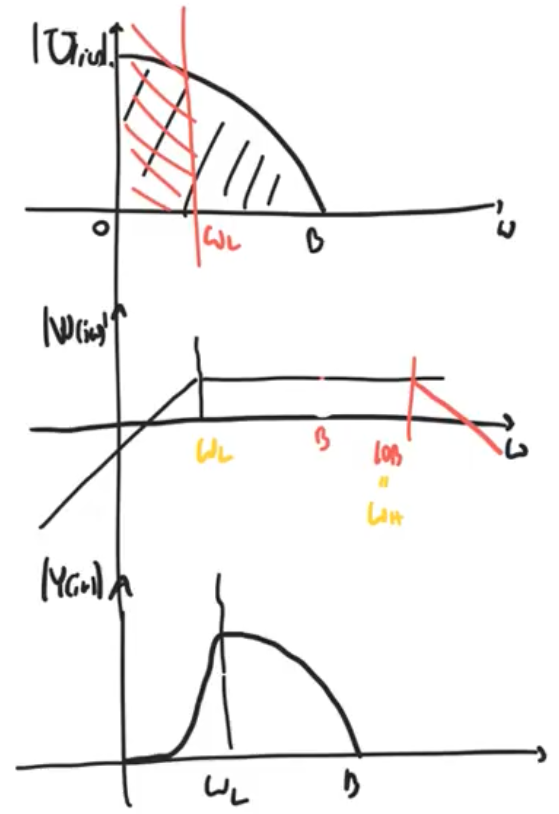
\includegraphics[width = 0.3\linewidth]{filtro_passa_alto}
\end{figure}
